
\chapter{Evaluating Generated Text}
\label{chap:evaluation}


In this chapter, we introduce two approaches for evaluating semantic accuracy of \ac{d2t} generation.

\section{Evaluating Semantic Accuracy}
\label{sec:sem-acc}

\begin{refbox}
    This section is based on the paper \emph{Evaluating Semantic Accuracy of Data-to-Text Generation with Natural Language Inference} \cite{dusekEvaluatingSemanticAccuracy2020}, joint work with Ondřej Dušek, published in the Proceedings of the The 13th International Conference on Natural Language Generation (INLG 2020). The experimental part was done by Ondřej Dušek, the author of this thesis came up with the initial idea and did the paper writing. The paper has received the award for the best short paper at the conference.
\end{refbox}

We propose a new metric for evaluating the semantic accuracy of D2T generation
based on a neural model pretrained for \ac{nli}. We use the \ac{nli} model to check textual entailment between the input data and the output text in both directions, allowing us to reveal omissions or hallucinations. Input data are converted to text for \ac{nli} using trivial templates. Our experiments on two recent D2T datasets show that our metric can achieve high accuracy in identifying erroneous system outputs. The experimental code for our metric is available on GitHub.\footnote{\url{https://github.com/ufal/nlgi_eval}}

\subsection{Motivation}
State-of-the-art neural \ac{d2t} generation models are prone to omitting or hallucinating facts \cite{gehrmanngehrmannEndtoEndContentPlan2018,ferrferreiraNeuralDatatotextGeneration2019,dusekEvaluatingStateoftheartEndtoEnd2020}, which restricts their real-world deployment. Recognizing these errors is thus essential for
proper system evaluation and further research in D2T generation.

In general, evaluating the semantic accuracy of D2T generation outputs requires full natural language understanding. Minor changes in wording may cause major differences in the meaning of the text, making it difficult for handcrafted heuristics to cover all edge cases. Human evaluation, on the other hand, is expensive and difficult to scale.

We note that the task of checking if a generated sentence includes/entails a particular fact is very close to the task of \ac{nli}. \ac{nli} is a sequence classification task which takes two inputs---a \textit{hypothesis} and a \textit{premise}---and produces one of the possible outputs: the hypothesis is \textit{entailed} by (follows from) the premise, \textit{contradicts} the premise, or their relation is \textit{neutral}. Recently, neural models for \ac{nli} \cite{zhang2019,liu-etal-2019-multi,liu_roberta_2019} reached near-human levels of performance and \ac{nli} was used for evaluating the output of abstractive summarization systems \cite{maynez-etal-2020-faithfulness}.

This brings a question: Can we use an \ac{nli} model for evaluating the semantic accuracy of D2T outputs?
The main idea of our method is to check with a general pretrained \ac{nli} model if the semantic information implied by the input data and the generated text is equal. We achieve this by using the \ac{nli} model to check for \textit{entailment} in two directions: By inferring input facts from the generated text we can check for \textit{omissions}, while the other direction allows us to check for \textit{hallucinations}.\footnote{This check in both directions is appropriate for D2T tasks that do not include content selection, which are the focus of our experiments in this paper. If the generator is supposed to select just some of the input facts to verbalize \cite[cf.~e.g.][]{wiseman_challenges_2017}, we can either only check for hallucinations or, if the content selection is explicit, perform a two-way check with the selected facts provided.}
For instance, consider the two input facts from Figure~\ref{fig:ex}: \emph{(Blue Spice | eat\_type | pub)}, \emph{(Blue Spice | area | riverside)} and the generated text: “You can bring your kids to Blue Spice in the riverside area.” A \ac{nli} system should detect that the first fact is not entailed by the text (there is no mention of Blue Spice being a pub), but the text is also not entailed by the facts (the information about kids is hallucinated).

Applying \ac{nli} for the D2T task brings a problem:
The hypothesis for the standard \ac{nli} task is a natural language text, but the input for D2T generation is structured. However, we show that we can easily sidestep this issue by transforming the data into text using a trivial template for each fact.

We demonstrate that even without any human references or in-domain training and with minimal handcrafting, our approach achieves high accuracy (>90\%) on the E2E Challenge data \cite{duvsek2020evaluating}, competitive with scripts specifically handcrafted for the domain, and produces useful results (>75\% accuracy, 0.6 Spearman correlation with human scores)
on the more challenging WebNLG dataset \cite{gardent2017webnlg}. A manual error analysis shows that some instances marked as errors were in fact assessed correctly by our metric; we also identified a few major sources of errors that can be mitigated by in-domain tuning.

\begin{figure*}[t]
    \centering
    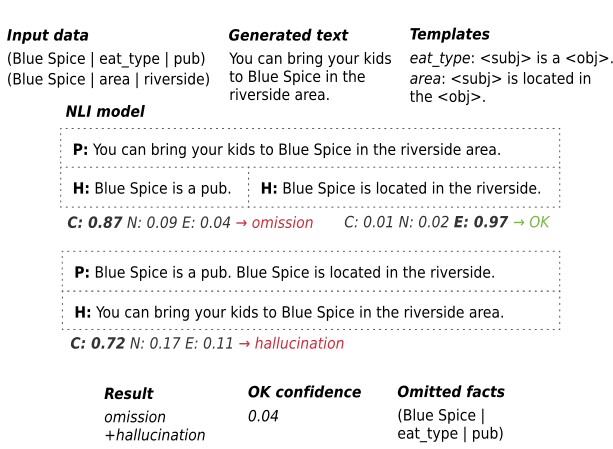
\includegraphics[width=\textwidth]{img/2020_nli_inlg}
    \caption{An example of evaluating the output from a D2T system with our metric. The generated text is used as a \textit{premise} (\textit{P}) to check for omissions and as a \textit{hypothesis} (\textit{H}) to check for hallucinations. The \ac{nli} model generates probabilities for \textit{contradiction} (\textit{C}), \textit{neutral} (\textit{N}) and \textit{entailment} (\textit{E}).}
    \label{fig:sem-acc:ex}
\end{figure*}
\paragraph{Automatic Evaluation of NLG} NLG outputs were traditionally evaluated by reference-based metrics measuring \emph{n}-gram overlap with a reference, such as BLEU \cite{papineni-etal-2002-bleu}, ROUGE \cite{lin-2004-rouge} and METEOR \cite{lavie_meteor:_2007}. Alternative, referenceless quality estimation metrics based on language model scores \cite{kann_sentence-level_2018} or linguistic features \cite{tian_treat_2018} focus on fluency and do not consider semantic accuracy. Recent works try to estimate NLG output quality with finetuned pretrained models \cite{zhou_learning_2020,zhang_bertscore:_2020,sellam_bleurt_2020}. The score from these models can capture some aspects of semantic accuracy, but only implicitly.

\paragraph{Semantic Accuracy}
To our knowledge, there is no generally accepted automatic metric for explicitly measuring semantic accuracy of NLG outputs. The closest commonly used metric is the \textit{slot error rate}, which is typically based on pattern matching tailored for a given dataset \cite{reed-etal-2018-neural,ijcai2019-437,duvsek2020evaluating}. Recently, \citet{goodrich_assessing_2019} introduced a metric based on training a neural model on named-entity recognition and fact extraction.

\paragraph{Faithful NLG}
Some recent neural NLG systems %of the works on neural NLG 
train specifically for semantic accuracy
%aim to make the output more faithful to the input 
\cite{nie-etal-2019-simple,tian2019sticking,kedzie-mckeown-2019-good}. Similarly to us, \citet{harkous2020have} use a pretrained neural model as a classifier to detect inaccurate output, finetuning the classifier on manually augmented domain-specific data.

Unlike previous works, we use a pretrained neural model finetuned for \ac{nli} which we do not further train on any domain-specific data.
\paragraph{Automatic Evaluation of NLG} NLG outputs were traditionally evaluated by reference-based metrics measuring \emph{n}-gram overlap with a reference, such as BLEU \cite{papineni-etal-2002-bleu}, ROUGE \cite{lin-2004-rouge} and METEOR \cite{lavie_meteor:_2007}. Alternative, referenceless quality estimation metrics based on language model scores \cite{kann_sentence-level_2018} or linguistic features \cite{tian_treat_2018} focus on fluency and do not consider semantic accuracy. Recent works try to estimate NLG output quality with finetuned pretrained models \cite{zhou_learning_2020,zhang_bertscore:_2020,sellam_bleurt_2020}. The score from these models can capture some aspects of semantic accuracy, but only implicitly.

\paragraph{Semantic Accuracy}
To our knowledge, there is no generally accepted automatic metric for explicitly measuring semantic accuracy of NLG outputs. % in terms of faithfulness to the input data. 
The closest commonly used metric is the \textit{slot error rate}, %for computing omissions, 
which is typically based on pattern matching tailored for a given dataset \cite{reed-etal-2018-neural,ijcai2019-437,duvsek2020evaluating}. Recently, \citet{goodrich_assessing_2019} introduced a metric based on training a neural model on named-entity recognition and fact extraction.

\paragraph{Faithful NLG}
Some recent neural NLG systems %of the works on neural NLG 
train specifically for semantic accuracy
%aim to make the output more faithful to the input 
\cite{nie-etal-2019-simple,tian2019sticking,kedzie-mckeown-2019-good}. Similarly to us, \citet{harkous2020have} use a pretrained neural model as a classifier to detect inaccurate output, finetuning the classifier on manually augmented domain-specific data.

Unlike previous works, we use a pretrained neural model finetuned for \ac{nli} which we do not further train on any domain-specific data.



\subsection{NLI model}
\label{sec:nli-model}
% No training needed
We use pretrained RoBERTa \cite{liu_roberta_2019} as implemented in the Transformers library \cite{wolf_huggingfaces_2020} for our \ac{nli} model. Specifically, we use the \texttt{roberta-large-mnli}\footnote{\scalebox{0.95}[1.0]{\url{https://huggingface.co/roberta-large-mnli}}} checkpoint, which was finetuned on the Multi\ac{nli} dataset \cite{williams-etal-2018-broad}. We use the model \textit{as is}, without any further training. %on our side.
Given a premise text and a hypothesis text, the \ac{nli} model produces a probability distribution over three results: \textit{contradiction}, % (the hypothesis contradicts the premise), 
\textit{neutral} %(the hypothesis does not contradict, but does not follow from the premise) 
and \textit{entailment} (cf.~Section~\ref{sec:intro}). % (the hypothesis follows from the premise).
We consider a \ac{nli} check as passed if the probability for \textit{entailment} is the highest of the three.

\subsection{Data Preparation}
\label{sec:templates}

% We focus on triple-like MRs, easy to represent others
The input to our metric is a set of facts (the input for a D2T system) and the corresponding verbalization of these facts (the output from a D2T system). In our setup, the facts are RDF-like triples in the \textit{subject-predicate-object} form.%\footnote{This can be easily extended to other similar data formats. (e.g., the E2E dataset was converted from attribute-value pairs for our experiments).}

We convert each triple
to natural language using a trivial template. We consider two cases:
\begin{enumerate}[nosep,label={(\arabic*)},leftmargin=14pt,labelwidth=12pt,labelsep=2pt]
    \item \emph{Default:} The templates can be handcrafted or extracted from the NLG systems' training data for each predicate.
    \item \emph{Backoff:} We use only a single, universal ``backoff'' template for all the facts, in the form: \emph{The \textless{}predicate\textgreater{} of \textless{}subject\textgreater{} is \textless{}object\textgreater{}}.
\end{enumerate}
Hereinafter, a \textit{fact} refers to a template filled with the values from the triple.


\subsection{Evaluation Process}
\label{sec:eval-process}

% Individual triples, take the max, must be E
The generated text is said to be correct if it mentions \textit{all} and \textit{only} the input facts.
We check if the text contains any omissions or hallucinations in two steps (see Figure~\ref{fig:ex} for an example):
\begin{enumerate}[nosep,label={(\arabic*)},leftmargin=14pt,labelwidth=12pt,labelsep=2pt]
    \item To check for omissions, we use the whole generated text as a premise and sequentially feed each fact as a hypothesis to the \ac{nli} model. Any failed \ac{nli} check is considered an omission. While we could use all concatenated facts in a single \ac{nli} check, our approach gives us further information about which facts are omitted.
    \item To check for hallucinations, we use a concatenation of all facts as a premise and feed the generated text as a hypothesis to the \ac{nli} model. If this \ac{nli} check fails, the text is considered to contain hallucination. This step cannot be split into simpler \ac{nli} checks.
\end{enumerate}
The final output of our metric is either 4-way (denoted as \textsc{Fine}): \emph{OK} (i.e., all \ac{nli} checks passed), \emph{omission}, \emph{hallucination} or \emph{omission+hallucination} (based on the failed checks), or 2-way (denoted as \textsc{Rough}) where the latter three results are collapsed into \emph{not\_OK}. The \textsc{Fine} 4-way output is more useful for system evaluation (we can distinguish whether the system tends to hallucinate or omit information). The \textsc{Rough} 2-way output corresponds more to a usage inside an NLG system for output reranking or filtering: any output that is \emph{not\_OK} should be penalized/\hspace{0mm}filtered out.
% Computing confidence: minimum for all
Additionally, we compute a \textit{confidence score} of the model as the minimum of all the entailment probabilities. %This score can serve as a measure of the model's confidence about the correctness of the generated text.


% =============================================================================
\section{Experimental Setup}
\label{sec:experiments}
% -----------------------------------------------------------------------------

% Two prominent recent data-to-text datasets



% Does have some problems, mostly related to domain (not family friendly -!> adult only, some random babble is hallucination...)

We experiment with two recent English data-to-text datasets with a triple-like format: WebNLG \cite{gardent2017webnlg} and E2E \cite{novikova-etal-2017-e2e}.\footnote{E2E data use attribute-value pairs relating to a restaurant; we convert them to triples where the restaurant is the subject.} Since both of them were used in shared tasks, sets of system outputs and measures of semantic accuracy are available (see Supplementary for details).
% Eval on WebNLG human rated, corr with humans
% No binary -> thresholding at 2.5 ()

For WebNLG, we compare our metric with crowdsourced human ratings of semantic adequacy \cite{shimorina2019webnlg}. %In particular, we use the question about semantic adequacy: \textit{Does the text correctly represent the meaning in the data?}, where the 
Human annotators used
%indicated the answer on 
a three-point Likert scale (1 = Incorrect, 2 = Medium, 3 = Correct) and answers are averaged over multiple annotators. In our experiments discussed in Section~\ref{sec:webnlg_results}, we consider a sentence correct if it achieved human rating 2.5 or higher (we also tried a threshold of 2.0, with slightly worse results).
% less accurate on humans
% but still quite OK. Since the domain is quite limited, this is possible to do.

For the E2E dataset, the challenge results were checked for semantic accuracy using a handcrafted automatic script \cite{duvsek2020evaluating},\footnote{While the E2E challenge did include crowdsourced evaluation of semantic accuracy, the results were unreliable, overestimating the number of errors \cite{duvsek2020evaluating}. Note that unlike our metric, such a handcrafted approach to evaluating semantic accuracy is only viable for limited domains such as E2E.%\OD{is the “unlike our metric” OK or too boastful?} \ZK{tak teď už všichni vidí, že se trefuješ sám do sebe, ne? :D mně to přijde ok, akorát je tu na mě moc poznámek pod čarou... co dát poznámku 4 do závorky do textu?}
} we therefore use this automatic script as the ground truth for evaluating our metric in Section~\ref{sec:e2e-results}.
We further use small sets of system outputs and human-written texts with expert annotation \citep[provided by][]{dusek_semantic_2019} to evaluate our approach against gold-standard annotation and to compare to existing semantic accuracy classifiers for E2E data in Section~\ref{sec:e2e-classifiers}.


We evaluate the \emph{Default} and \emph{Backoff} approaches to acquiring templates as described in Section~\ref{sec:templates}. The \emph{Default} setup works with one custom template per predicate type. For WebNLG, we obtained templates by delexicalizing human references for single-triple examples from WebNLG training data.\footnote{For each predicate, we choose randomly if more templates are found and use the backoff if no templates are found.} For E2E, we handcrafted 8 templates.
The templates are filled with values from individual input triples and concatenated for multi-triple inputs as described in Section~\ref{sec:eval-process}. %\OD{is this OK? they're not concatenated for omission checks; OTOH R\#1 didn't really get this and thought we can only handle 1-triple WebNLG stuff} \ZK{jo, myslím, že je to takhle pochopitelný}


% There's also limited human-annotated system outputs (400) and human-written scripts (200),
% where we can compare to the automatic script.

% =============================================================================
\section{Results Analysis}
\label{sec:results}
% -----------------------------------------------------------------------------


\begin{table}[t]
    \centering \small
    \begin{tabular}{l ccccc} \toprule
                & \textbf{A} & \textbf{R} & \textbf{P} & \textbf{F1} & $\mathbf{\rho}$ \\\midrule
        Default & 0.775      & 0.772      & 0.796      & 0.784       & 0.628           \\
        Backoff & 0.768      & 0.760      & 0.793      & 0.776       & 0.637           \\ \bottomrule
    \end{tabular}
    \caption{WebNLG dataset results, compared to crowdsourced human ratings (A = accuracy, R = recall, P = precision, F1 = F-measure, $\rho$ = Spearman correlation of confidence scores with human scores).}
    \label{tab:webnlg}
\end{table}

\begin{table}[t]
    \centering \small
    \begin{tabular}{l cccccc} \toprule
                & \textbf{Af} & \textbf{Ar} & \textbf{R} & \textbf{P} & \textbf{F1} \\\midrule
        Default & 0.911       & 0.933       & 0.895      & 0.910      & 0.903       \\
        Backoff & 0.846       & 0.874       & 0.913      & 0.768      & 0.834       \\
        \bottomrule
    \end{tabular}
    \caption{E2E dataset results, compared to the automatic evaluation script %The experiments on the second lines ignore \textit{eatType=restaurant}. 
        (Af = \textsc{Fine} accuracy, Ar = \textsc{Rough} accuracy, R = recall, P = precision, F1 = F-measure).}
    \label{tab:e2e}
\end{table}


\begin{table*}[t]
    \centering\footnotesize
    \begin{tabular}{@{}l c c ccc >{\hspace{3mm}} c c ccc@{}}\toprule
                          & \multicolumn{5}{c}{\bfseries Human-written (E2E training set)} & \multicolumn{5}{c}{\bfseries System outputs (TGen)}                                                                     \\
                          & \bf Af                                                         & \bf Ar                                              & \bf R & \bf P & \bf F1 & \bf Af & \bf Ar & \bf R & \bf P & \bf F1 \\\midrule
        Slug2Slug aligner & 0.685                                                          & 0.765                                               & 0.550 & 0.800 & 0.652  & 0.995  & 1.000  & 1.000 & 1.000 & 1.000  \\
        %                              & 0.920 & 0.930 & 0.977 & 0.764 & 0.857 & 0.990 & 0.995 & 1.000 & 0.947 & 0.973 \\
        E2E script        & 0.820                                                          & 0.885                                               & 1.000 & 0.777 & 0.874  & 0.995  & 0.995  & 1.000 & 0.950 & 0.974  \\
        %                              & 0.615 & 0.700 & 1.000 & 0.417 & 0.589 & 0.990 & 0.990 & 1.000 & 0.900 & 0.947 \\
        TGen reranker     & 0.110                                                          & 0.435                                               & 0.975 & 0.413 & 0.579  & 0.220  & 0.278  & 1.000 & 0.116 & 0.208  \\
        %                              & 0.100 & 0.270 & 1.000 & 0.228 & 0.371 & 0.218 & 0.273 & 1.000 & 0.110 & 0.198 \\ 
        \midrule
        % TGen rer. cls. (cleaned data) & 0.155 & 0.415 & 0.988 & 0.405 & 0.574 & 0.338 & 0.403 & 1.000 & 0.138 & 0.241 \\
        %   & 0.100 & 0.240 & 1.000 & 0.221 & 0.361 & 0.338 & 0.398 & 1.000 & 0.130 & 0.230 \\\midrule
        Default           & 0.600                                                          & 0.700                                               & 0.625 & 0.625 & 0.625  & 0.978  & 0.978  & 0.947 & 0.837 & 0.888  \\ % 005
        %                              & 0.765 & 0.805 & 0.976 & 0.525 & 0.683 & 0.983 & 0.983 & 1.000 & 0.837 & 0.911 \\ % 007
        Backoff           & 0.530                                                          & 0.640                                               & 0.675 & 0.540 & 0.600  & 0.833  & 0.833  & 0.974 & 0.359 & 0.525  \\\bottomrule % 006
        %                              & 0.665 & 0.705 & 0.977 & 0.420 & 0.587 & 0.835 & 0.835 & 1.000 & 0.353 & 0.522 \\\bottomrule % 008
    \end{tabular}
    \caption{Semantic classifiers evaluated on expert human annotation on E2E data (see Table~\ref{tab:e2e} for metrics legend).} %; second line ignores eatType=restaurant}
    \label{tab:e2e-slot-comparison}
\end{table*}



% Random baseline would be 0.5 or 0.25 for fine
We evaluate our metric in terms of accuracy, precision, recall, and F1-measure (where \emph{not\_OK} samples are treated as positive since we focus on detecting errors).
We additionally perform a manual error analysis on a random sample of 100 error examples for each dataset, i.e.\ examples where our metric gave a different assessment from the ground truth (provided by crowdsourced annotation for WebNLG and by a handcrafted classification script for E2E as described in Section~\ref{sec:experiments}). % \ZK{zase bych dal poznámku klidně do textu, ať čtenář nemusí tolik skákat}
In general, the results are high above the random baseline (0.5 for the \textsc{Rough} metric and 0.25 for the \textsc{Fine} metric) but differ between the datasets, which we discuss below. %in the following subsections.



% The results for the E2E dataset are better, probably due to the lower lexical variability of the dataset.
% \OD{a možná kvůli tomu, že human eval pro webnlg je trochu zašuměný, ale nevim, jestli se to sem hodí}


% recall is probably more important than precision (not that there are differences)

\subsection{WebNLG Analysis}
\label{sec:webnlg_results}
The overall scores for the WebNLG dataset are summarized in Table \ref{tab:webnlg}. %Here, we compare the \textsc{Rough} metric against the (thresholded) human rating.
To further check whether the size of the input affects performance, we computed Spearman correlation of the number of input triples with metric errors. The resulting very low value of -0.05 ($p=$\,0.02, \emph{Default} setting) shows that the metric holds its performance even for more complex WebNLG examples. %\OD{added this, does it work here?} \ZK{chvilku mi trvalo pochopit, co to číslo počítá, ale asi jo}
%\OD{number of predicates doesn't seem to have a huge effect on performance (1: 78.22, 2: 84.00, 3: 73.55, 4: 77.55, 3: 73.95; spearman -0.0503, p=0.0175)}

%
%
% WebNLG much worse, although still better than random
% not much difference with the backoff templates -- 0.77 vs 0.76
% good correlation with human judgements 0.62-0.63
%
% We can see that the setup using only a backoff template leads to almost the same results as the default setup.
%
%\OD{TODO supplementary should have examples}
%\OD{not much difference w.r.t. backoff means templates are bad}
On the other hand, the overall scores show that our metric deviates quite a lot from the human judgments. Our manual error analysis indicates several reasons for that (see Supplementary for examples): (1) The annotation is somewhat noisy and using a threshold is not ideal---many correctly rendered outputs do not reach the 2.5 threshold (while some incorrect ones do). (2) Imprecise templates can confuse the \ac{nli}
%make the metric check for different information 
(e.g., for the predicate \emph{nationality}, our extracted template is \emph{\textless{}subj\textgreater{} was \textless{}obj\textgreater{}}, which works well with values such as \emph{French}, but not with \emph{United States}). This is currently a weak point of our metric, as illustrated by the very small performance difference between the \emph{Default} and \emph{Backoff} setups; however, the issue can be mitigated by a better selection of the templates from training data, e.g.\ using language-model scoring.
(3) The human annotators tend to give lower scores to accurate but ungrammatical or poorly organized texts. Our metric tends to rate these texts as \emph{OK}.
%Third, we note that many examples are dubious, e.g. there are typos in the text or the text interprets the data too loosely. In these cases, the notion of semantic accuracy can differ between the annotators.
Overall, our re-examination shows that almost half of the error examples (42 out of 100) were in fact correctly classified by our metric (i.e.\ their crowdsourced human annotation was incorrect), %\ZK{přidat něco jako "and not by human evaluators", ať je z toho jasný, že se díváme na chyby a tvrdíme, že to vlastně nejsou chyby?}\OD{takhle dobrý?}
so the true performance is most likely higher than the reported numbers. % due to errors in human annotation.

The Spearman correlation of our model's confidence scores with the average human scores is around 0.63 ($p<$1e-10). This is similar to n-gram-based metrics on this data (\citealp{shimorina_human_2018} reports 0.59 for BLEU and 0.73 for METEOR), but unlike these metrics, our approach does not require human-written reference texts.



\subsection{E2E Analysis}
\label{sec:e2e-results}

% E2E -- very good result -- 0.9 rough, 0.92 fine

% below average prices =~ less than £20
% adult only != not family friendly

% noticeable difference w.r.t. backoff templates

The results for the E2E dataset (shown in Table \ref{tab:e2e}) are very good compared to the WebNLG dataset, with over 90\% agreement with the handcrafted script. This can be attributed to lower lexical variability and less noisy texts, as well as to the better quality of the handcrafted templates (the difference between the \emph{Default} and \emph{Backoff} setups is much more pronounced here).
Again, we observe only a very slight drop in performance for more complex E2E inputs (Spearman correlation of metric errors with the number of input triples is -0.08, $p<$1e-10 for the \emph{Default} setting).
%\OD{only slight drop in performance for more complex inputs (around 96\% rough for up to 5 triples, 93\% for 6 triples, 91\% for 7, spearman 0.07638, p=1.3948e-18)}

%The reference texts often ignore \textit{eatType=restaurant}, which is probably deemed as implicit for the domain. We report the results where we ignore this particular slot-value pair and we observe notable improvements.
%\OD{TODO remove this, incl. from tables}
%\OD{TODO bigger diff w.r.t. backoff, i.e. templates are better}
The main issues identified by our error analysis are:
(1) Problems in the interpretation of some values, e.g., \textit{price range=less than \textsterling{}20} is verbalized as ``cheap'' or \textit{family-friendly=no} as ``adult-only''. These cases are classified as \emph{not\_OK} by the \ac{nli} model.
(2) Missing or over-greedy patterns in the slot error script, causing annotation errors.
(3) Edge cases: some expressions cannot be interpreted in a straightforward way, e.g.\ ``high restaurant'' for \emph{pricerange=high} is deemed OK by the \ac{nli} but not by the slot error script.
(4) Expressions in the outputs that do not correspond to input facts, such as ``with full service'', are considered hallucinations by the \ac{nli}, but ignored by the slot error script.
Again, we consider about half of the error examples (45 out of 100) as correctly classified by our metric (see Supplementary for details), and thus our metric's performance is probably higher than the reported values due to erroneous annotation from the handcrafted script.

% - - - - - - - - - - - - - - - - - - - - - - - - - - - - - - - - - - - - - -
\subsection{E2E MR Classifier Comparison}
% - - - - - - - - - - - - - - - - - - - - - - - - - - - - - - - - - - - - - -
\label{sec:e2e-classifiers}
%As described in Section~\ref{sec:experiments}, there are data in the E2E restaurant domain human-annotated for accuracy (part of the training set, some TGen outputs; \citealp{dusek_semantic_2019}). 
We used expert-annotated E2E data samples (%part of the training set and some system outputs, 
cf.~Section~\ref{sec:experiments}) to compare our approach to other accuracy classifiers in the E2E domain:
\begin{itemize}[nosep,leftmargin=10pt]
    \item \textbf{Slug2Slug slot aligner} \citep{juraska_deep_2018} is based on keyword matches. It is carefully tuned but not designed to detect hallucination; it only checks for presence of facts from the input MR.
    \item \textbf{E2E slot error script} (used in Section~\ref{sec:e2e-results}) is based on regular expressions; it is also able to detect irrelevant facts.
    \item \textbf{TGen reranker} is an LSTM-based model trained on the E2E training data to rerank outputs of the TGen system \cite{dusek_sequence--sequence_2016} based on their semantic accuracy.
          % \item TGen's reranking classifier trained on cleaned E2E data (i.e., reclassified by the slot error script)
\end{itemize}

The results for all classifiers (in Table~\ref{tab:e2e-slot-comparison}) are much weaker on human-written data, which exhibit much more variability than system outputs.
%While the TGen reranker may be useful for relative comparisons of system outputs, it 
The TGen reranker is very weak when required to detect all facts properly.
Our approach is slightly less precise than both handcrafted scripts, but the difference is small on system outputs (97.8\% vs. 99.5\% accuracy). If we disregard the value \emph{eatType=restaurant}, which is generally noisy, we get 76.5\% accuracy and 97.6\% recall on the human-written data. Moreover, our approach requires much less handcrafting and is more general.


\section{Token-Level Error Detection}
\label{sec:eval-token}
\subsection{Shared Task}
\label{sec:eval-st}
\subsection{Our Submission}
\label{sec:eval-ours}